
Here, we describe the outcomes of the preregistered simulations.
Overall, the performance of \ainet{} was virtually identical to elastic net
regression. The adaptive penalization weights of \ainet{} do not seem to make a
difference for the data generating mechanism considered in our simulations.
Moreover, since the data were generated under a process equivalent to a logistic
regression model, it is no surprise that for reasonably large sample sizes,
logistic regression also performed the best. The only exception are
conditions with small sample size and low number of events per variable. Here,
\ainet{} and elastic net led to more stable and better calibrated predictions
than logistic regression. The random forest was outperformed by \ainet{} in most
simulation conditions, with exception of very small sample size and prevalence,
as well as when a high correlation between covariates was present. Finally, the
performance of the adaptive elastic net was generally worse compared to
\ainet{} and elastic net. In the following, we summarize the results for each
estimand.

%%%%%%%%%%%%%%%%%%%%%%%%%%%%%%%%%%%%%%%%
\subsection{Brier score (primary estimand)}
%%%%%%%%%%%%%%%%%%%%%%%%%%%%%%%%%%%%%%%%
Figure~\ref{fig:tiebrier} shows the differences in mean Brier score between
\ainet{} and the other methods stratified by simulation conditions.
% elastic net
We see that there is hardly any difference between \ainet{} and the elastic net (EN)
across all simulation conditions meaning that predictive performance of both
methods seems to be very similar in the investigated scenarios.

% random forest
The random forest (RF) shows better predictive performance than \ainet{} in
conditions with very low sample size ($n = 100$) and prevalence
($\mbox{prev} = 0.01$). For increasing sample size and prevalence, the
performance of \ainet{} seems to become more similar or improve over RF when the
correlation of the covariates is not too large ($\rho \leq 0.6$) especially for
low events per variable ($\mbox{EPV} \leq 1$). For highly correlated covariates
($\rho = 0.95$), the performance of \ainet{} is similar or worse across most
simulation conditions.

% GLM
Logistic regression (GLM) showed better predictive performance compared to
\ainet{} in most simulation conditions. An exception are the conditions with
small sample size ($n = 100$), medium to large prevalence
($\mbox{prev} \geq 0.05$) and low events per variable ($\mbox{EPV} \leq 1$),
where \ainet{} performed better than GLM.

The adaptive elastic net (AEN) method performed worse than \ainet{} in almost
all simulation conditions. Only in conditions with very large sample size
($n = 5000$), very small prevalence ($\mbox{prev} = 0.01$), and high events per
variable ($\mbox{EPV} = 20$), AEN showed predictive performance on par with
\ainet{}.

%%%%%%%%%%%%%%%%%%%%%%%%%%%%%%%%%%%%%%%%
\subsection{Scaled Brier score (secondary estimand)}
%%%%%%%%%%%%%%%%%%%%%%%%%%%%%%%%%%%%%%%%
Figure~\ref{fig:tiesbrier} shows the differences in scaled Brier score between
\ainet{} and the other methods stratified by simulation conditions. The scaled
Brier score is useful to compare the actual values of Brier scores across
conditions with different prevalence, but not so much to compare Brier scores of
different methods within a simulation condition with fixed prevalence.

We see that for most conditions the plots look like a flipped version of the
original Brier scores from Figure~\ref{fig:tiebrier}. Therefore, conclusions are
mostly the same. For very small sample sizes coupled with low prevalence and low
events per variable (the topleft plots), the scaled Brier score indicates
superiority of \ainet{} over RF and GLM, which is opposite the conclusion based
on the raw Brier score. We advise to interpret these conditions cautiously since
the prevalence prediction which is used for scaling is based on the much larger
test data set.

%%%%%%%%%%%%%%%%%%%%%%%%%%%%%%%%%%%%%%%%
\subsection{Log-score (secondary estimand)}
%%%%%%%%%%%%%%%%%%%%%%%%%%%%%%%%%%%%%%%%
Figure~\ref{fig:tienll} shows the differences in log-score between \ainet{} and
the other methods stratified by simulation conditions. We see that in certain
conditions, the error bars of certain methods are much larger. This is due to
the log-score's sensitivity to extreme predictions, which often happen under the
RF (and sometimes under the GLM). Despite the larger variability of the log-score,
conclusion regarding the comparison between \ainet{} and the other
methods are largely the same as under the Brier score.

%%%%%%%%%%%%%%%%%%%%%%%%%%%%%%%%%%%%%%%%
\subsection{Area under the curve (secondary estimand)}
%%%%%%%%%%%%%%%%%%%%%%%%%%%%%%%%%%%%%%%%
Figure~\ref{fig:tienll} shows the differences in area under the curve (AUC)
between \ainet{} and the other methods stratified by simulation conditions.
As with the other estimands, \ainet{} shows virtually identical performance
as EN regression across all simulation conditions.
\ainet{} seems to outperform RF across most simulation conditions, with the
exception of a conditions with low sample size ($n = 100$), medium prevalence
($\mbox{prev} = 0.05$), and low events per variable ($\mbox{EPV} \leq 1$).
GLM, typically outperforms \ainet{} conditions with small to medium sample size
($n \leq 500$), and also in conditions with larger sample size when the
events per variable is normal to high ($\mbox{EPV} \geq 10$) and the prevalence
is small ($\mbox{prev}  = 0.01$).
Finally, the AEN is worse with respect to AUC than \ainet{} across all
simulation conditions.

%%%%%%%%%%%%%%%%%%%%%%%%%%%%%%%%%%%%%%%%
\subsection{Calibration slope (secondary estimand)}
%%%%%%%%%%%%%%%%%%%%%%%%%%%%%%%%%%%%%%%%
Figure~\ref{fig:cslope} shows boxplots of calibration slopes stratified by
simulation condition and method. For each condition the percentage of
simulations where no estimate could be obtained is indicated. This usually
happened because of extreme (close to zero or one) predictions, or
non-convergence of the method itself. We caution against interpretation of the
random forest (RF) calibration slopes because this method often resulted in
predicted probabilities of zero or one, so that a calibration slope could not
be fitted.

We see that logistic regression (GLM) shows on average optimal calibration slopes
in most simulation condition. In cases where it is off one, its calibration
slopes are usually too small indicating overoptimistic predictions. In general,
worse calibration slopes are obtained for lower event per variable (EPV).

The penalized methods (\ainet{}, EN, AEN) show a more stable behavior, and on
average larger calibration slopes than GLM. This is likely confounded by the
simulation conditions in which no GLM calibration slope can be estimated, but
estimation of the penalized methods' calibration slope is still possible. Among
the penalized method's \ainet{} and EN shows relatively similar calibration
slopes whereas the AEN shows worse calibration slopes that are more off the
value of one.

%%%%%%%%%%%%%%%%%%%%%%%%%%%%%%%%%%%%%%%%
\subsection{Calibration in the large (secondary estimand)}
%%%%%%%%%%%%%%%%%%%%%%%%%%%%%%%%%%%%%%%%
Figure~\ref{fig:clarge} shows boxplots of calibration in the large estimates
stratified by simulation condition and method. For each condition also the
percentage of simulations where no estimate could be obtained is indicated.
This usually happened because of extreme (close to zero or one) predictions.

We see that the number of simulations with non-estimable calibration is
substantially larger when the sample size is small, whereas it decreases for
larger sample sizes. An exception is the RF where the number of non-estimable
calibrations stays high across most conditions.

While all methods seem to be marginally well calibrated, the penalized methods
(\ainet{}, EN, and AEN) show lower numbers of simulations with non-estimable
calibration compared to GLM, especially for low to medium sample sizes and low
events per variables.

%---%---%---%---%---%---%---%---%---%---%---%---%---%---%---%---%---%---%---%---%---
\begin{landscape}
\begin{figure}[!ht]
\center
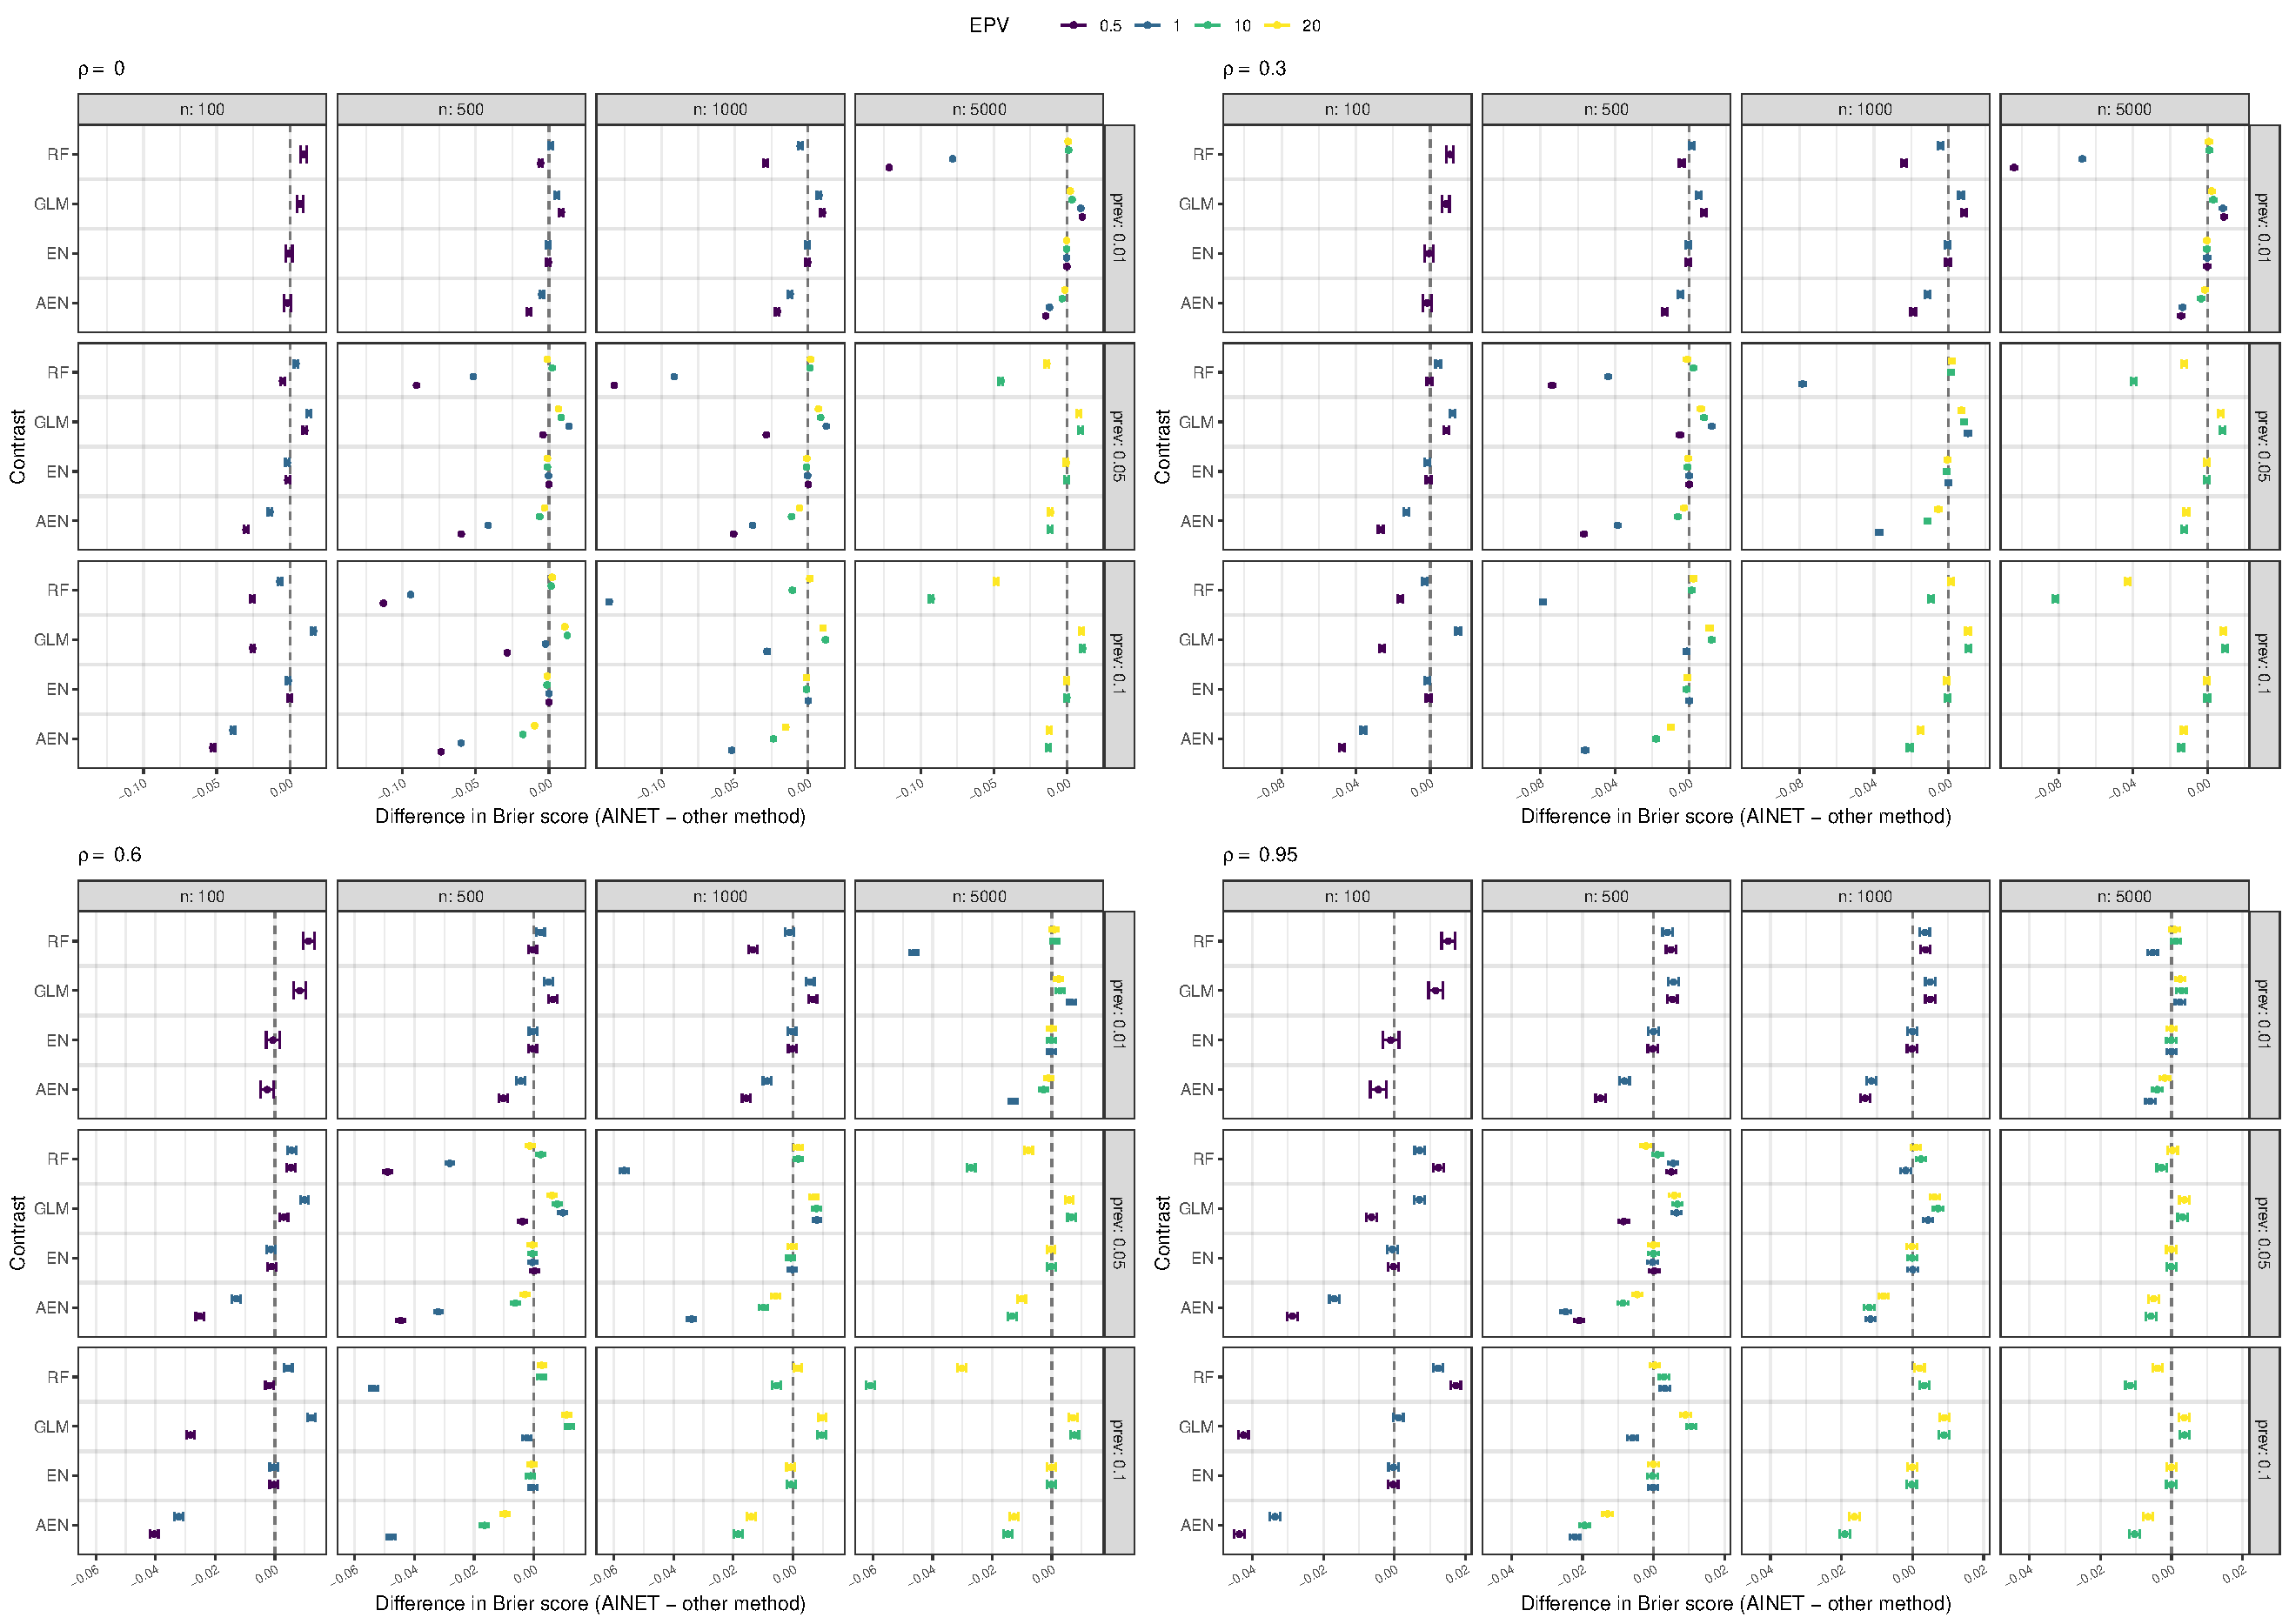
\includegraphics[width=0.9\linewidth]{figures-appendix/tie-fighter_brier.pdf}
\caption{Tie-fighter plot for the difference in Brier score between any method
  on the $y$-axis and \ainet{}. The 95\% confidence intervals are adjusted per
  simulation condition using the single-step method. Lower values indicate
  better performance of \ainet{}. } \label{fig:tiebrier}
\end{figure}
\end{landscape}
%---%---%---%---%---%---%---%---%---%---%---%---%---%---%---%---%---%---%---%---%---

%---%---%---%---%---%---%---%---%---%---%---%---%---%---%---%---%---%---%---%---%---
\begin{landscape}
\begin{figure}[!ht]
\center
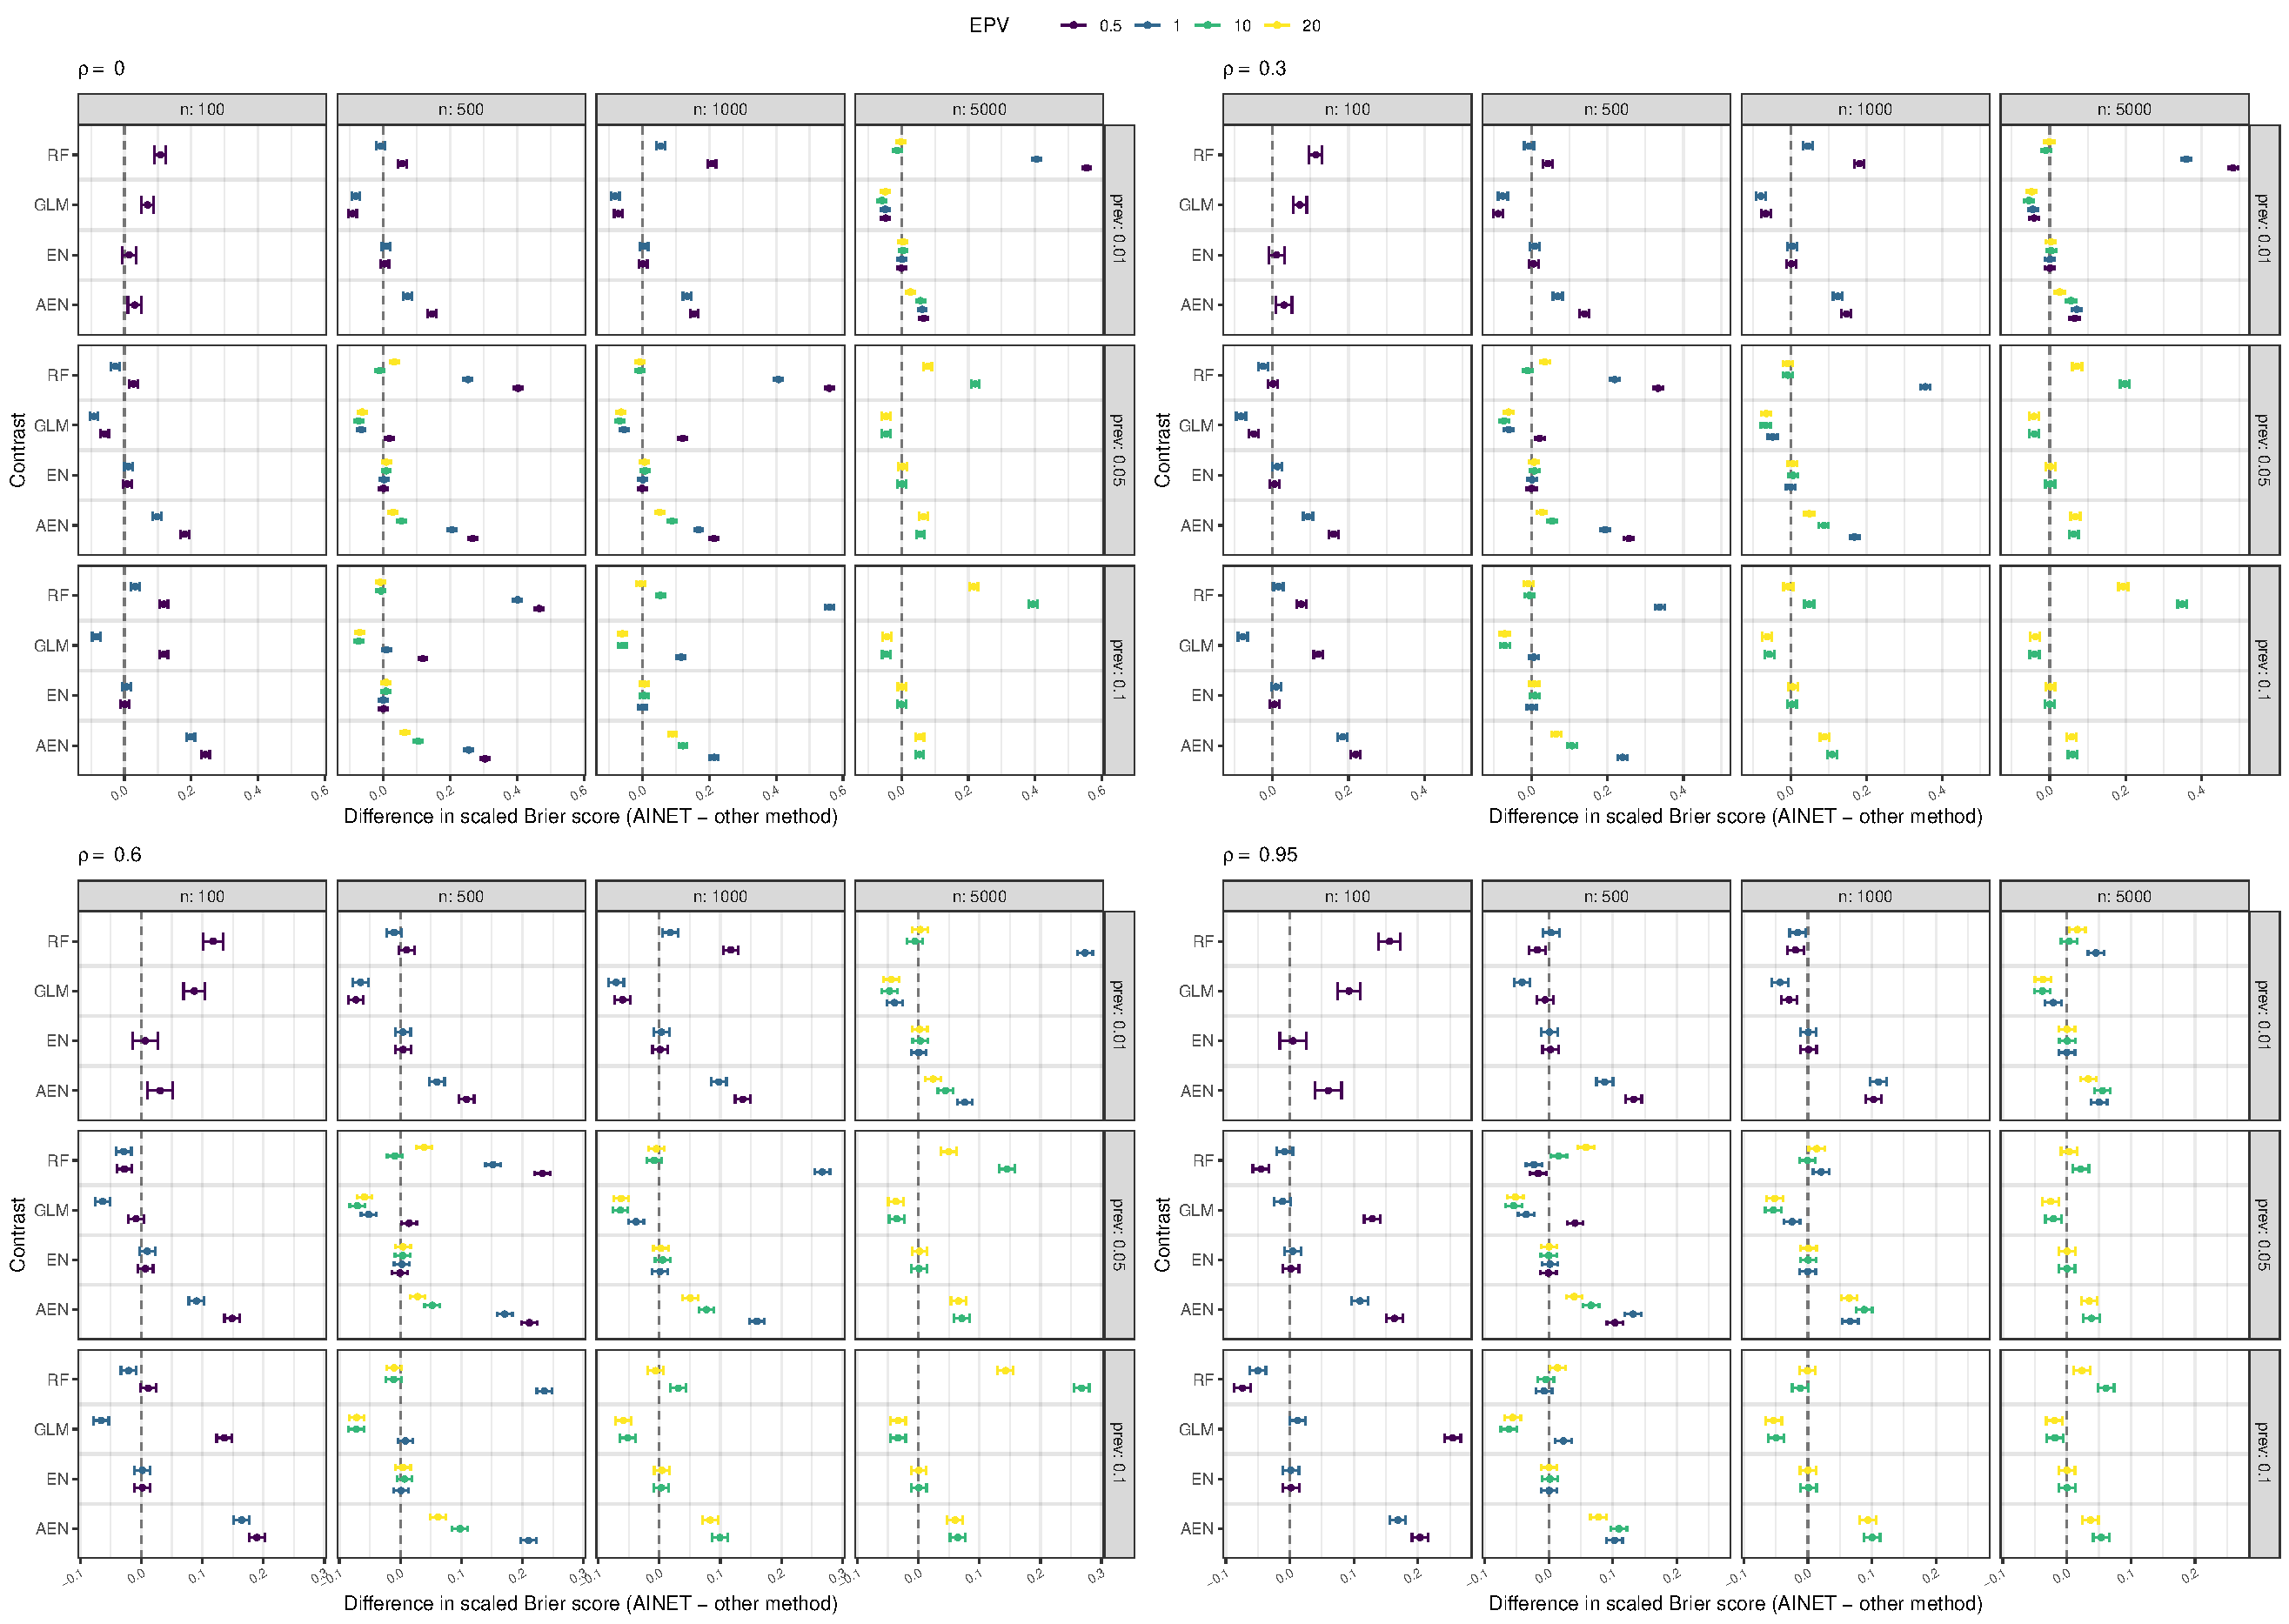
\includegraphics[width=0.9\linewidth]{figures-appendix/tie-fighter_scaledBrier.pdf}
\caption{Tie-fighter plot for the difference in scaled Brier score between any
  method on the $y$-axis and \ainet{}. The 95\% confidence intervals are adjusted
  per simulation condition using the single-step method. Larger
  values indicate better performance of \ainet{}. } \label{fig:tiesbrier}
\end{figure}
\end{landscape}
%---%---%---%---%---%---%---%---%---%---%---%---%---%---%---%---%---%---%---%---%---

%---%---%---%---%---%---%---%---%---%---%---%---%---%---%---%---%---%---%---%---%---
\begin{landscape}
\begin{figure}[!ht]
\center
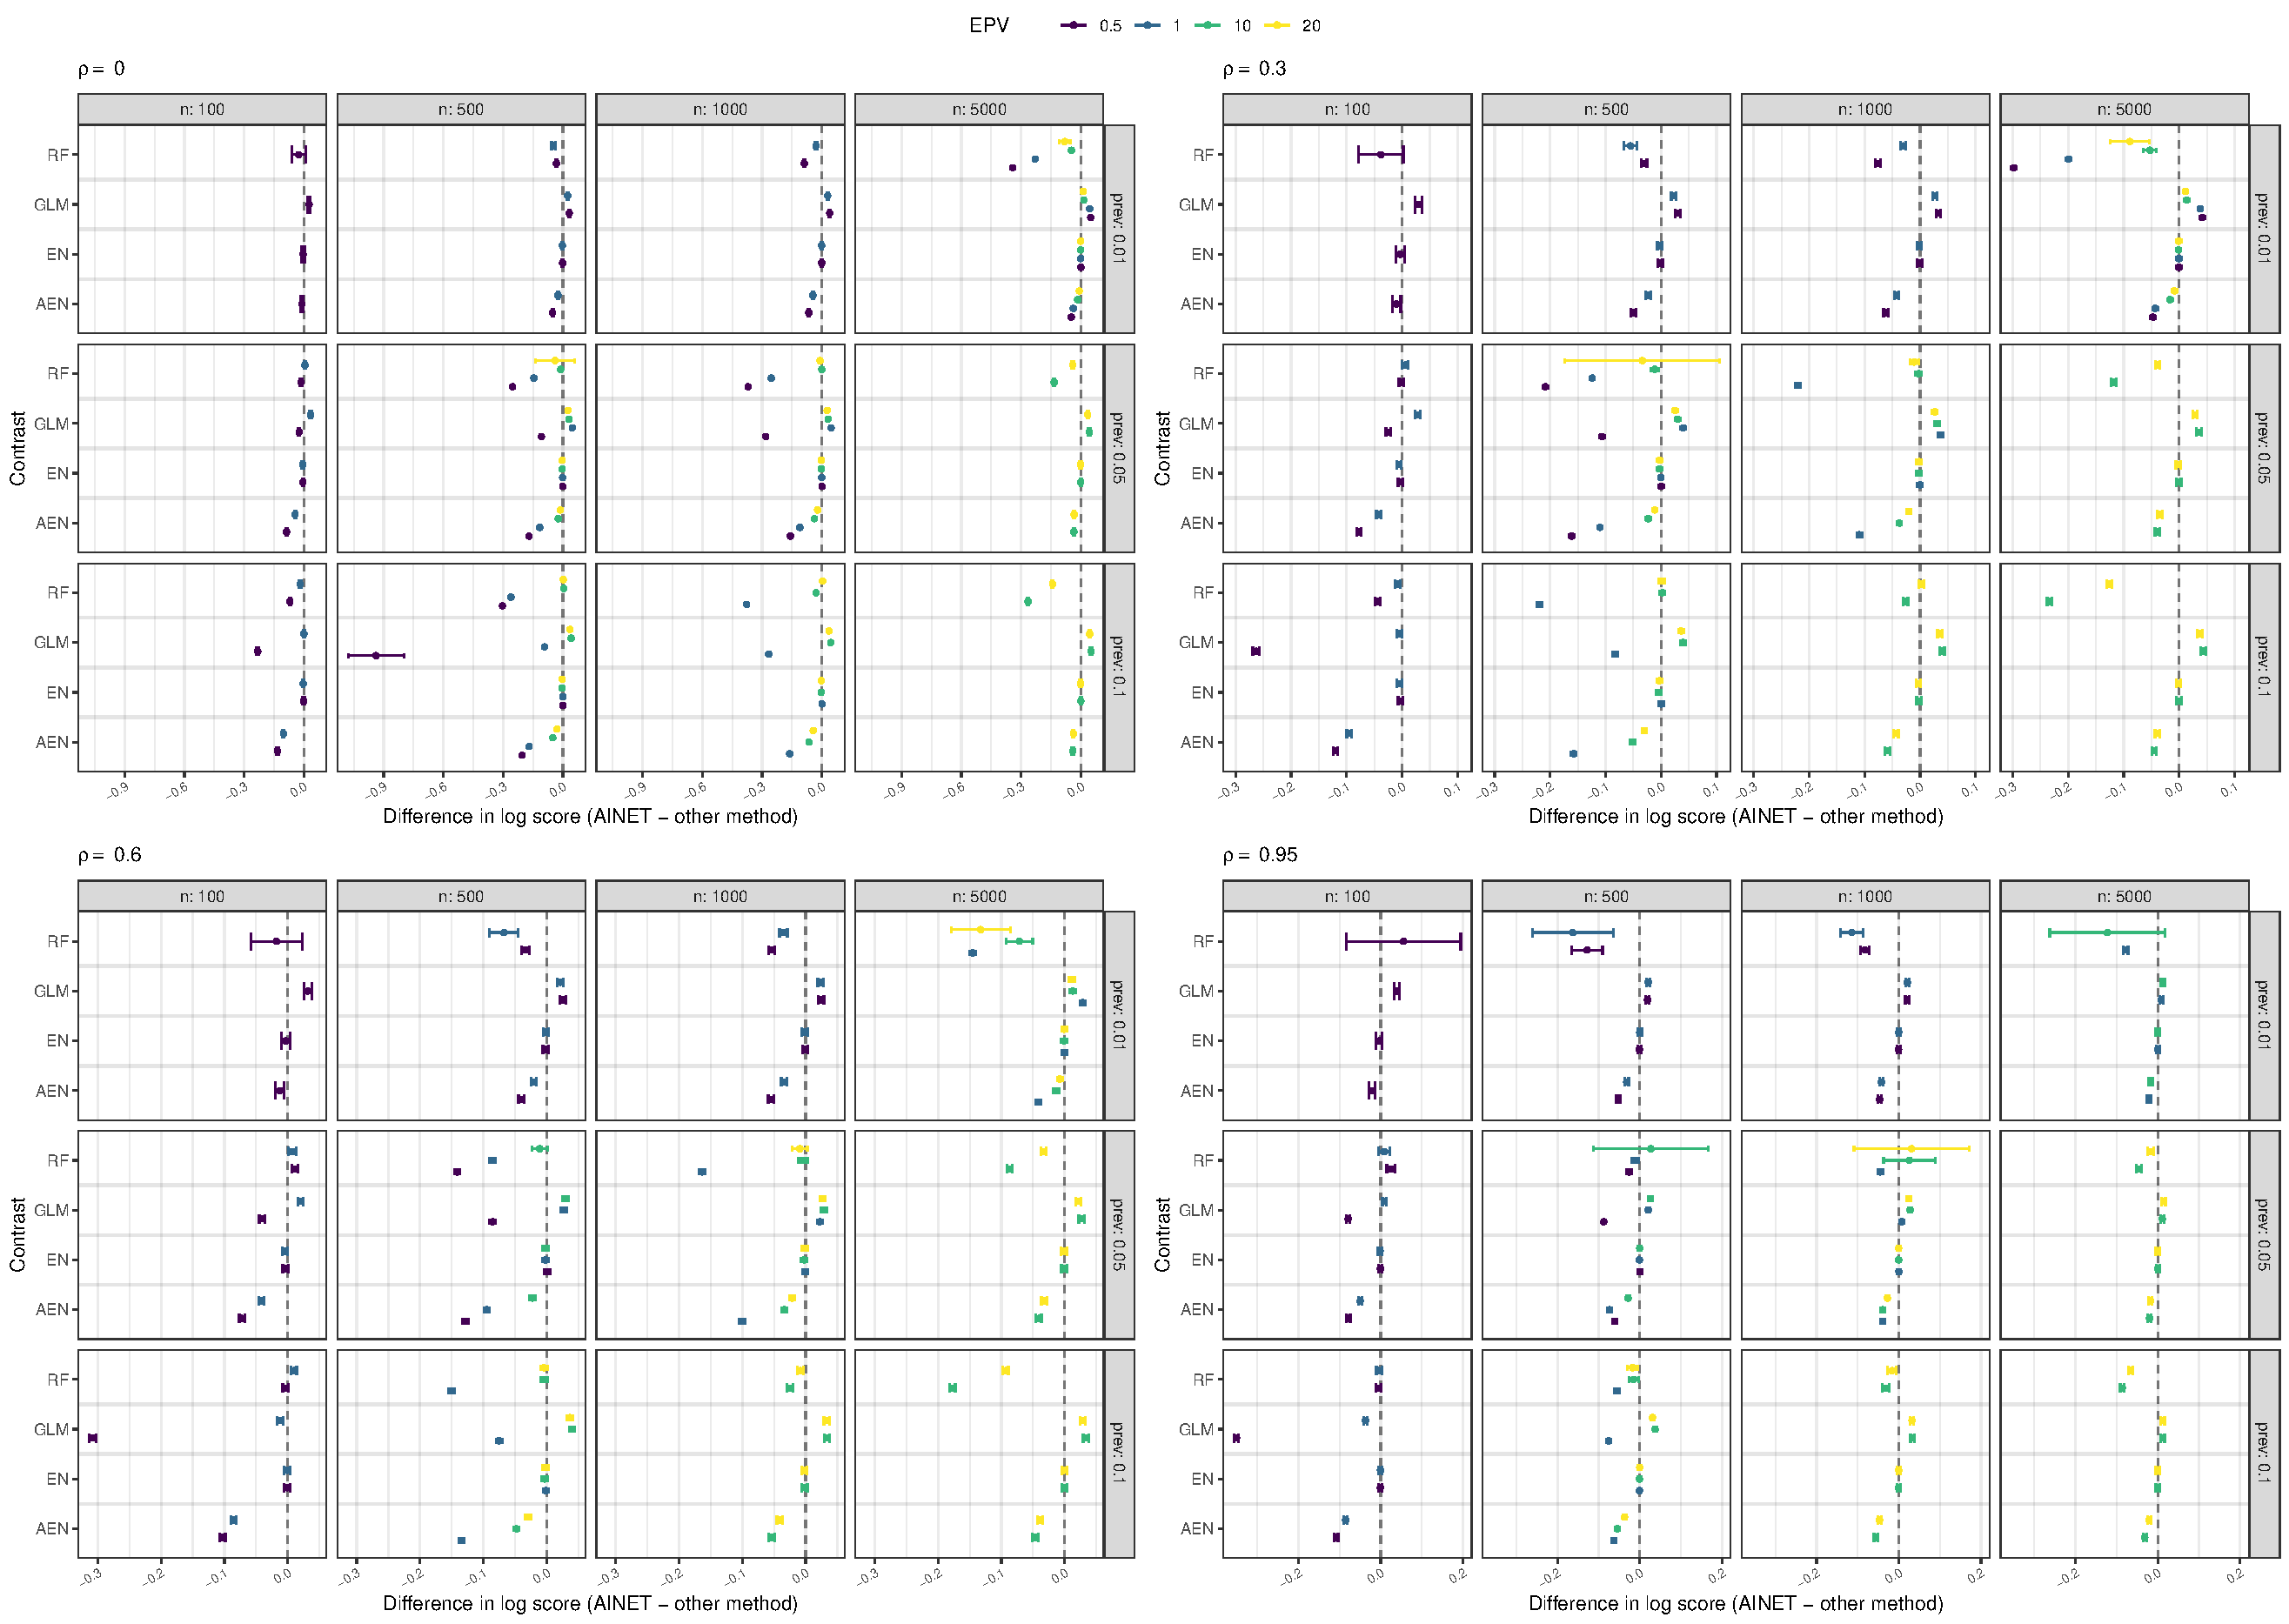
\includegraphics[width=0.9\linewidth]{figures-appendix/tie-fighter_nll.pdf}
\caption{Tie-fighter plot for the difference in log-score between any method on
  the $y$-axis and \ainet{}. The 95\% confidence intervals are adjusted per
  simulation condition using the single-step method. Lower values indicate
  better performance of \ainet{}. } \label{fig:tienll}
\end{figure}
\end{landscape}
%---%---%---%---%---%---%---%---%---%---%---%---%---%---%---%---%---%---%---%---%---

%---%---%---%---%---%---%---%---%---%---%---%---%---%---%---%---%---%---%---%---%---
\begin{landscape}
\begin{figure}[!ht]
\center
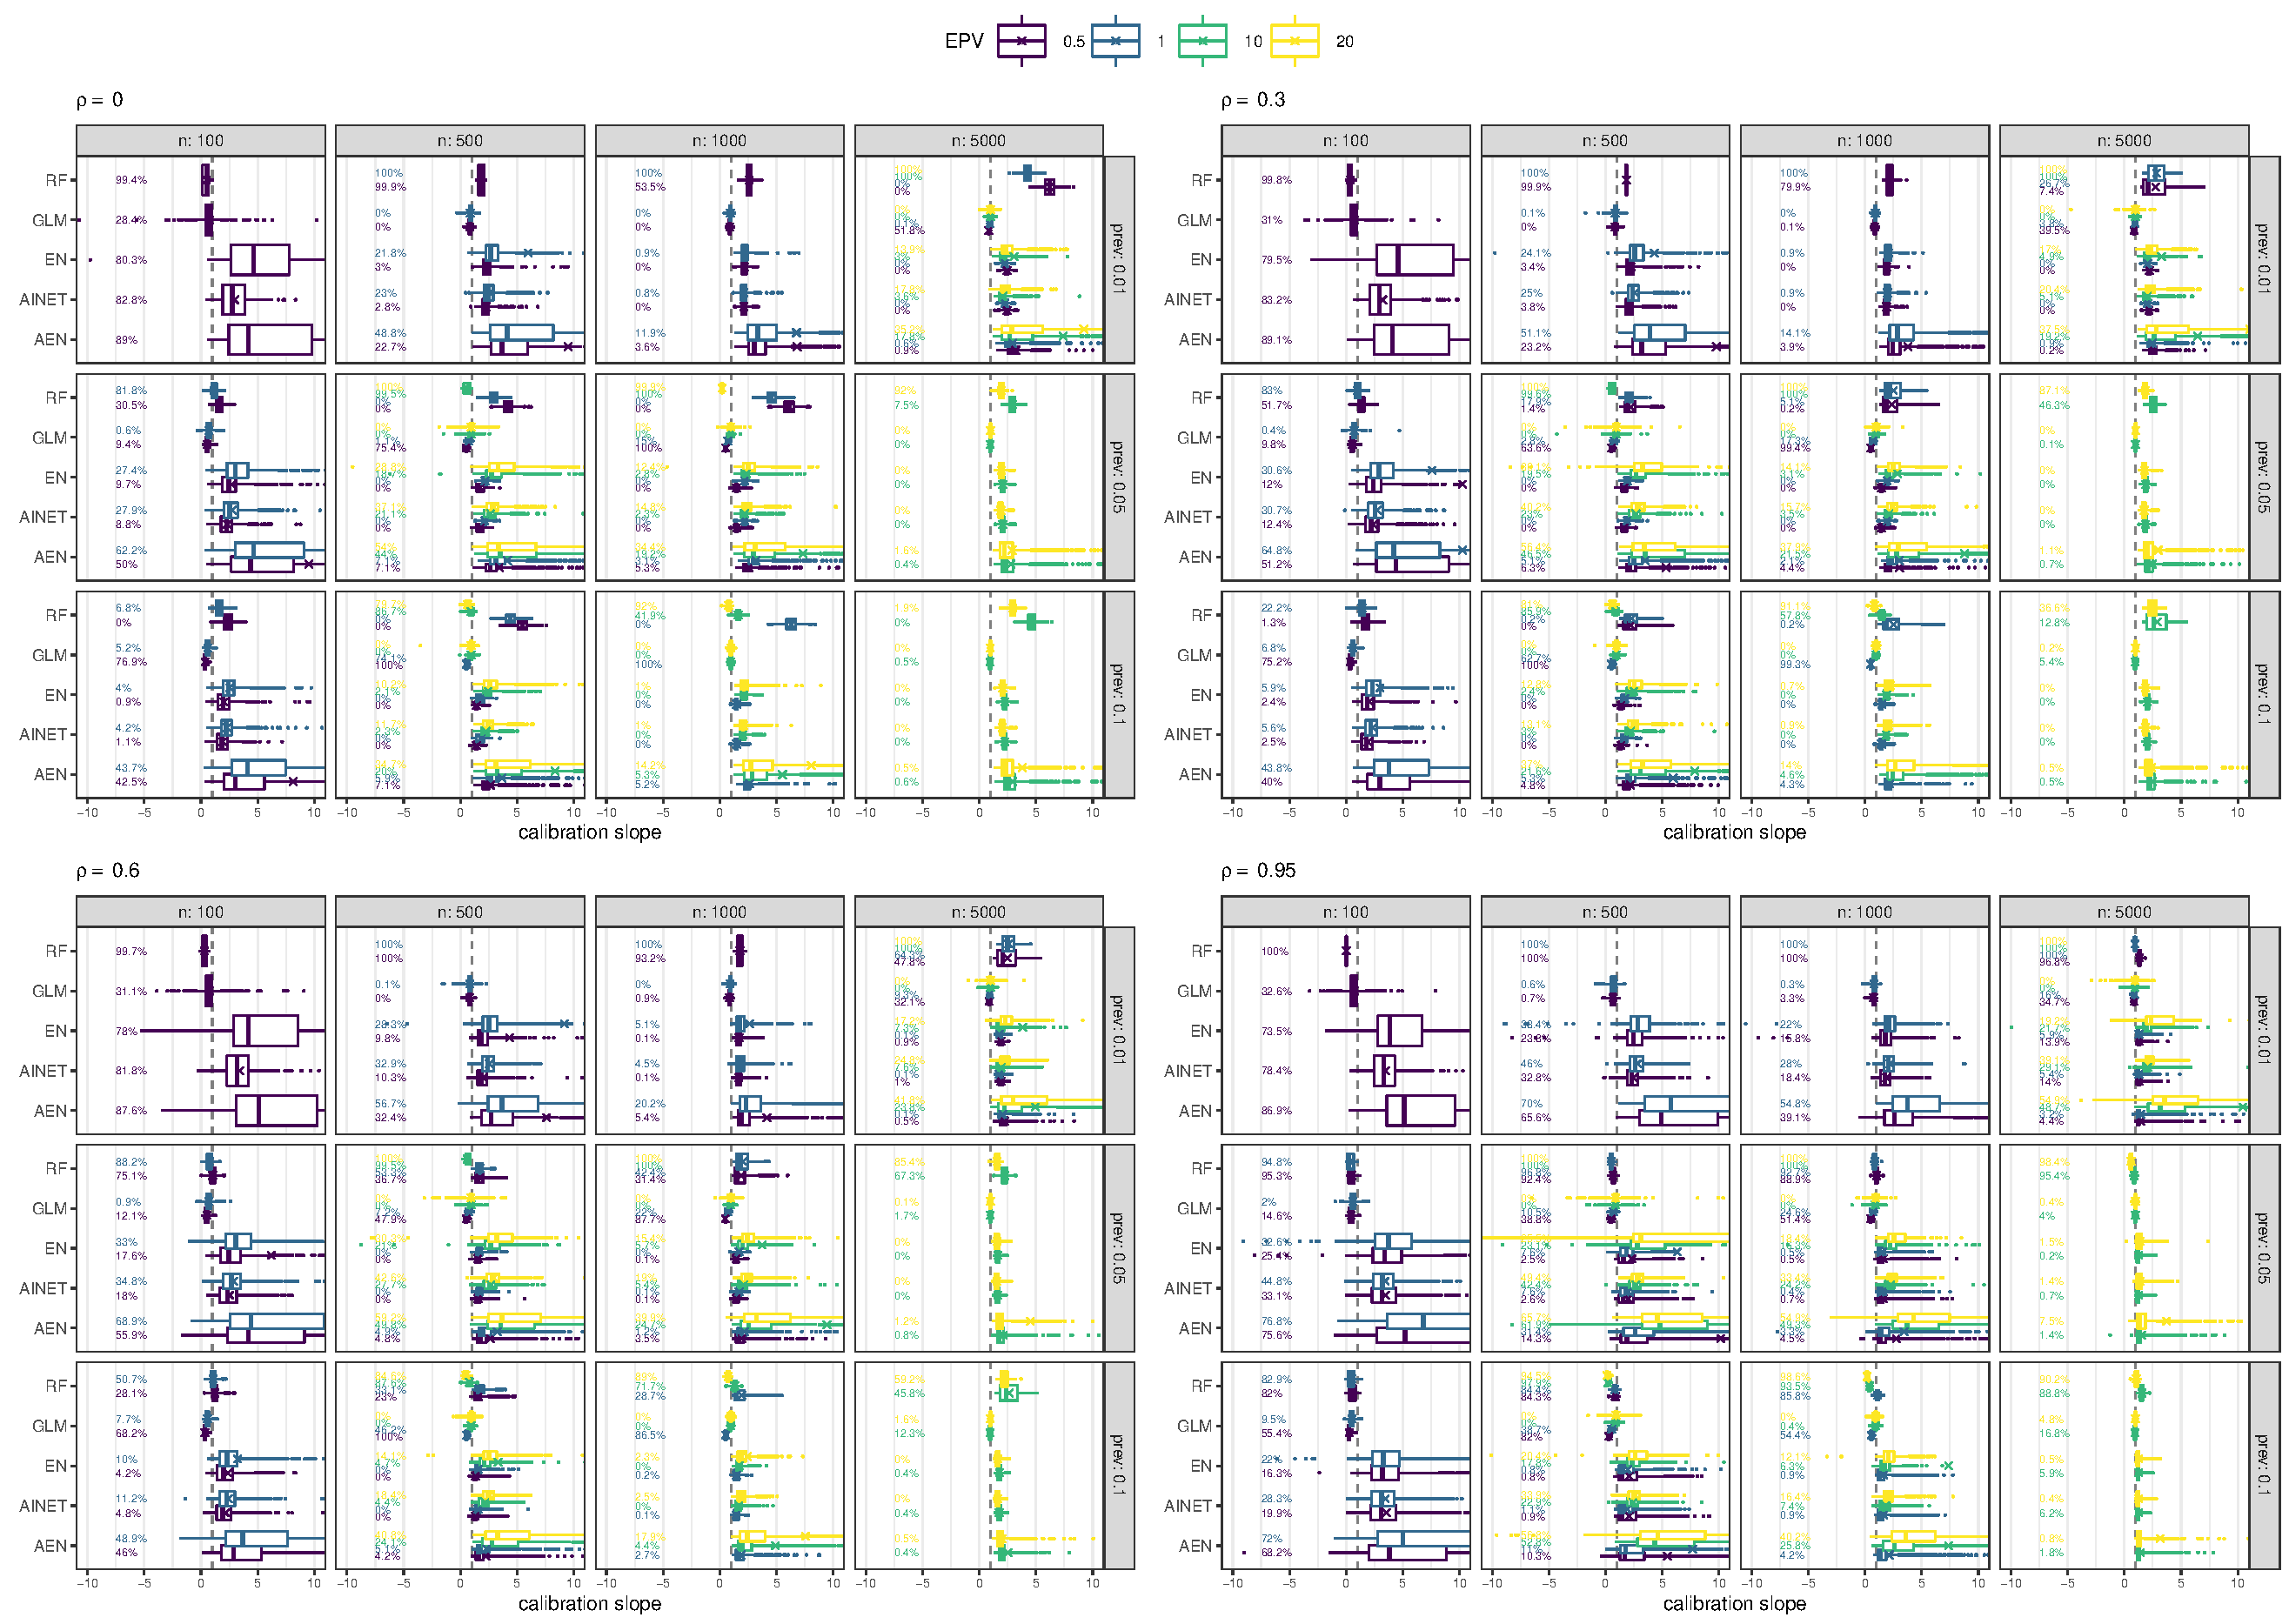
\includegraphics[width=0.9\linewidth]{figures-appendix/calibration-cslope.pdf}
\caption{Boxplots of calibration slopes stratified by method and simulation
  conditions. Mean calibration slope is indicated by a cross. A value of one
  indicates optimal calibration. Percentage of simulations where calibration
  slope could not be estimated (due to extreme predictions or complete
  separation) are also indicated.} \label{fig:cslope}
\end{figure}
\end{landscape}
%---%---%---%---%---%---%---%---%---%---%---%---%---%---%---%---%---%---%---%---%---

%---%---%---%---%---%---%---%---%---%---%---%---%---%---%---%---%---%---%---%---%---
\begin{landscape}
\begin{figure}[!ht]
\center
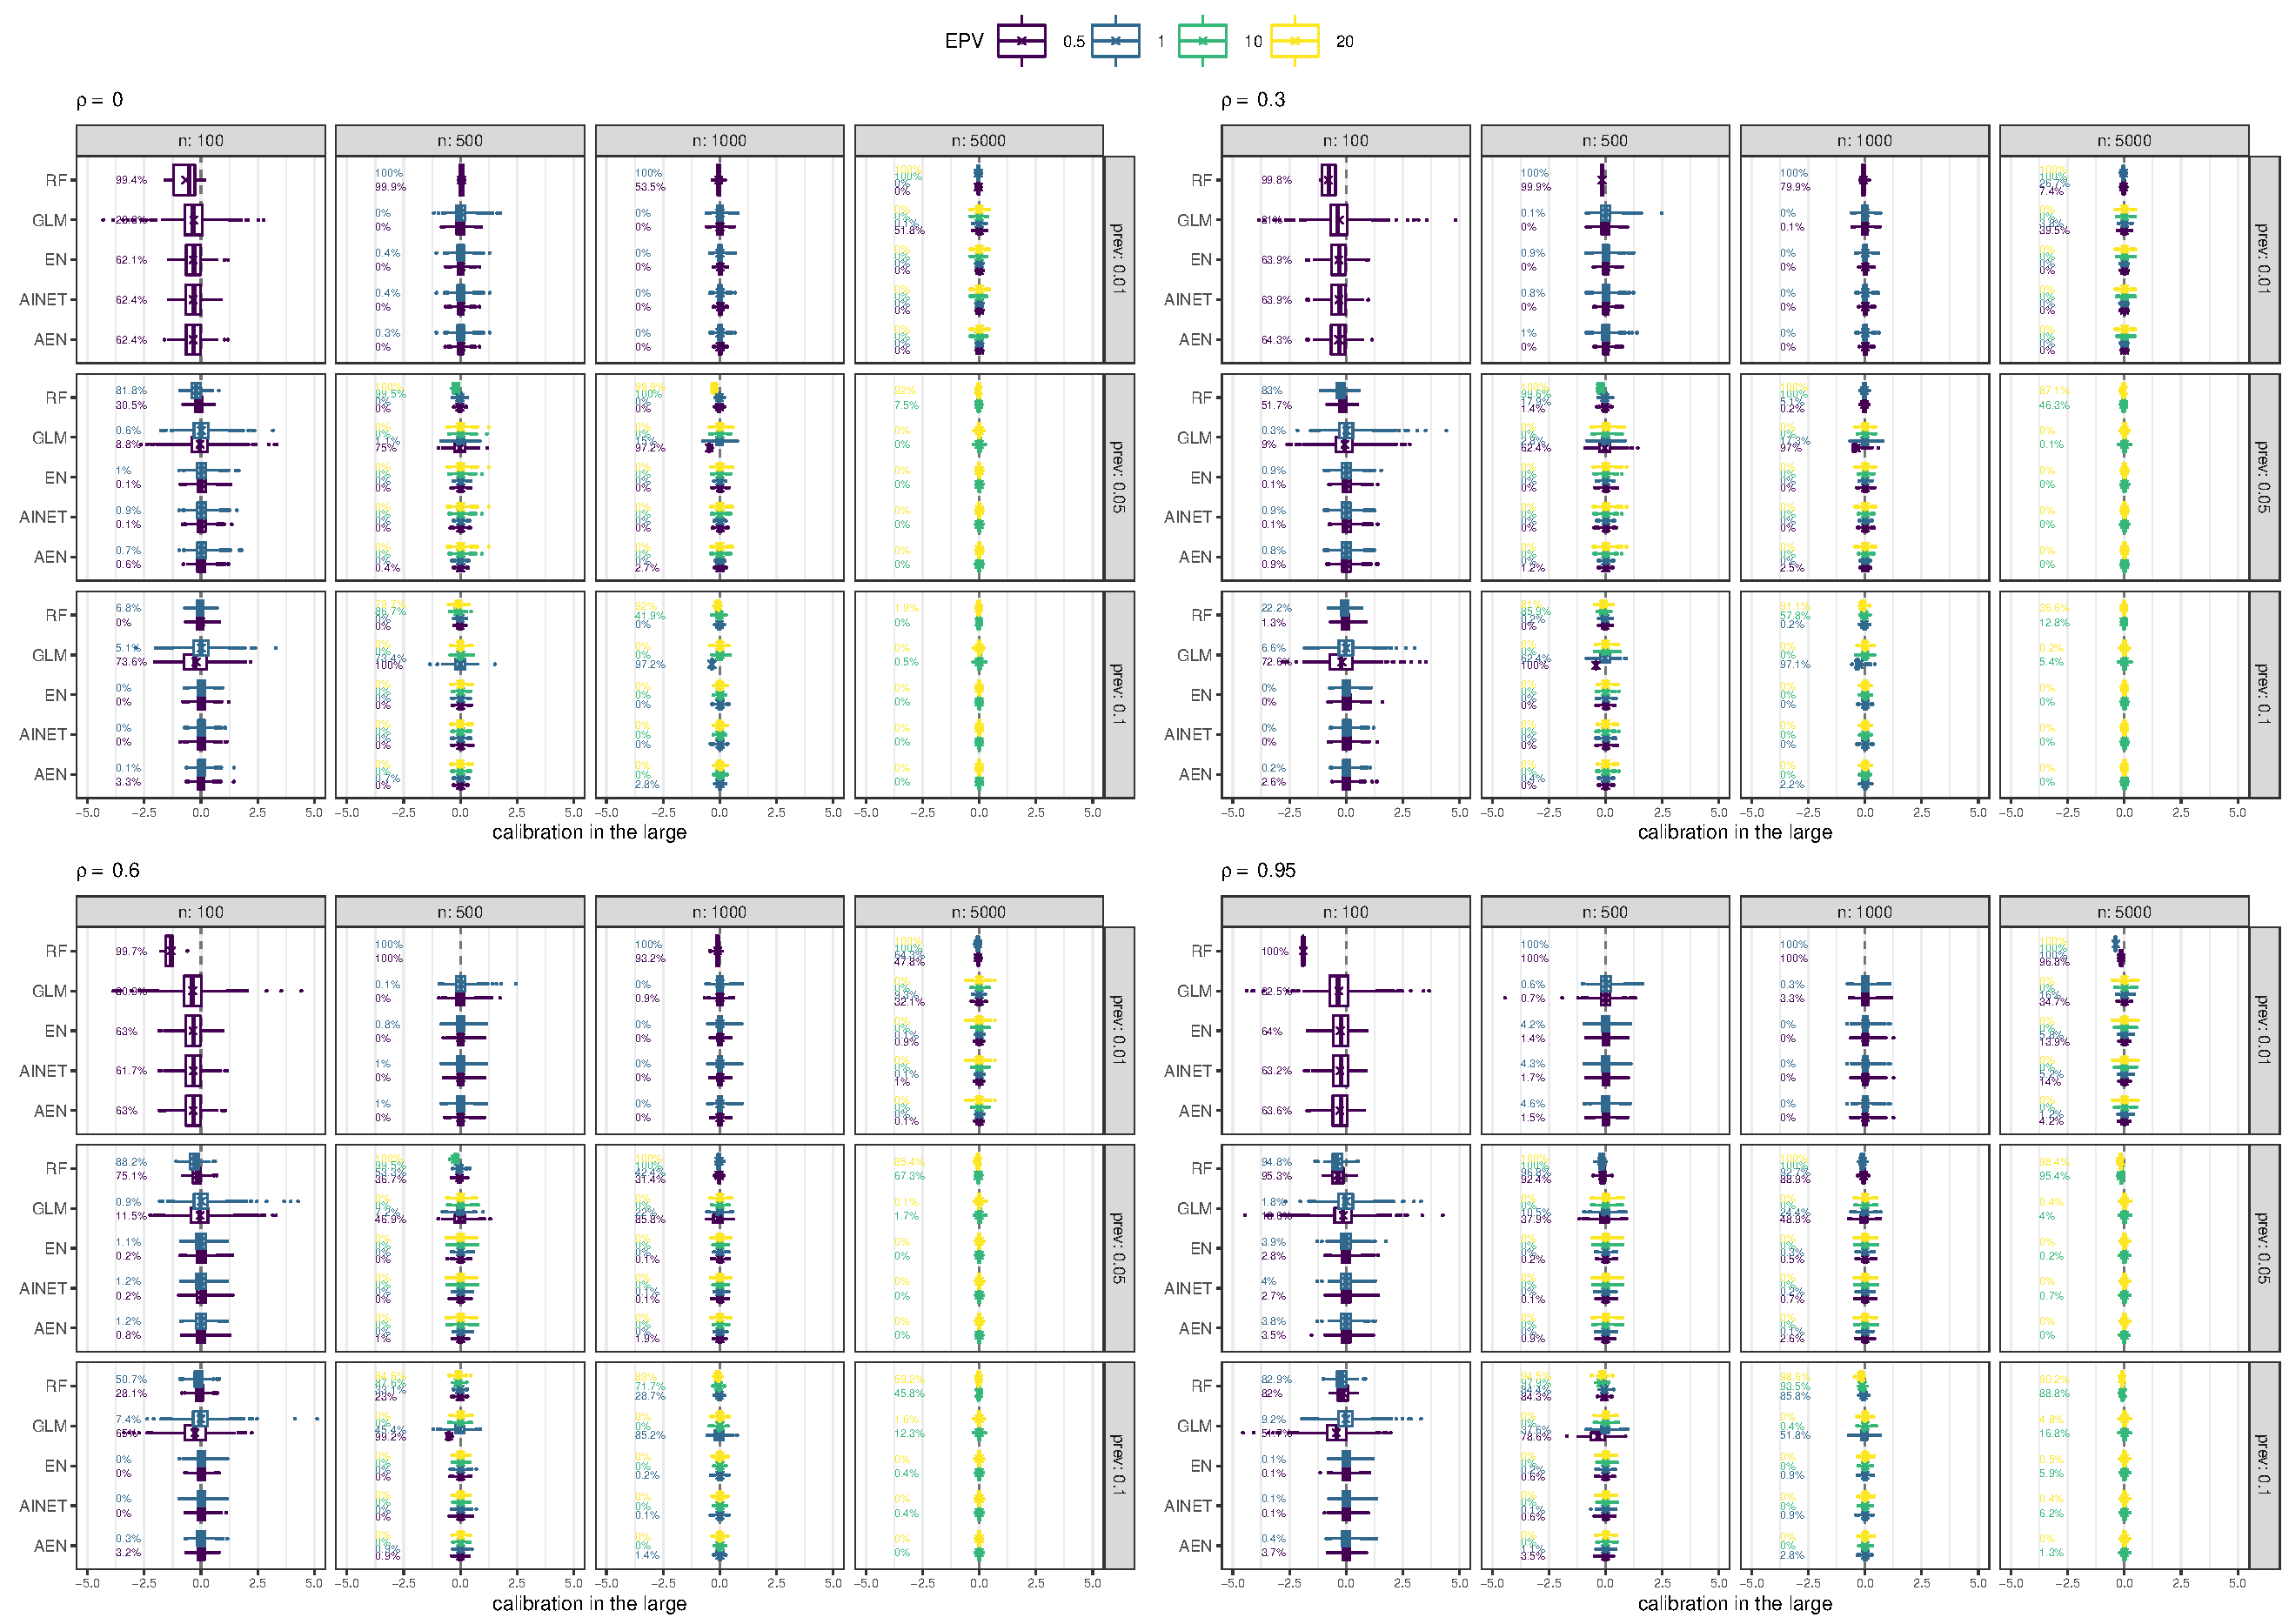
\includegraphics[width=0.9\linewidth]{figures-appendix/calibration-clarge.pdf}
\caption{Boxplots of calibration in the large stratified by method and
  simulation conditions. Mean calibration in the large is indicated by a cross.
  A value of zero indicates optimal calibration in the large. Percentage of
  simulations where calibration in the large could not be estimated (due to
  extreme predictions or complete separation) are also
  indicated.} \label{fig:clarge}
\end{figure}
\end{landscape}
%---%---%---%---%---%---%---%---%---%---%---%---%---%---%---%---%---%---%---%---%---
